\documentclass{article}

\usepackage{polski}
\usepackage[utf8]{inputenc}
\usepackage{graphicx}
\usepackage{float}

\title{\Huge{
		\indexspace Projekt zespołowy \\[1cm] 
		\indexspace Aplikacja internetowa do zarządzania finansami 
		\indexspace \textbf{"Where's my money?!"}}}

\author{Patryk Mroczyński \and Oskar Rutkowski \and Jakub Wiśniewski}

\begin{document}
	
	\pagenumbering{gobble}
	\maketitle
	\newpage
	\tableofcontents
	\newpage
	\pagenumbering{arabic}
	
	\section{Charakterystyka ogólna projektu}
	\paragraph{} Aplikacja ma na celu uproszczenie zarządzania budżetem domowym użytkownika. Umożliwia ona dodawanie wydatków i przychodów wraz z przypisaniem im odpowiednich kategorii. Dodawanie może odbywać się albo jako importowanie pliku w formacie CSV, który jest generowany przez użytkownika na stronie banku, albo poprzez ręczne wpisanie przez użytkownika kwoty i przydzielenia kategorii. Użytkownik może definiować subkonta, do których przypisywane są wydatki. Aplikacja umożliwia generowanie raportów i wykresów dla określonego przedziału czasowego z uwzględnieniem tylko wybranych kategorii czy subkont, które są wybrane przez użytkownika. Użytkownik ma możliwość eksportowania raportów do wybranego formatu.
	\section{Architektura systemu}
	\paragraph{} System oparty jest na modelu klient-serwer, gdzie klient (łącznie z interfejsem i logiką po stronie klienta) jest uruchamiany w przeglądarce, a na maszynie serwerowej działa relacyjna baza danych oraz program, który wykonuje operacje na bazie danych i udostępnia API, z którego korzysta aplikacja kliencka. Serwer składa się z mikrousług, które udostępniają metody zgodnie z architekturą REST. \\[0.5cm]
	Serwer składa się z mikroserwisów, które udostępniają odpowiednie metody protokołu HTTP dla klienta.
	
	\subsection{Mikroserwisy}
	W podrozdziale zostały wylistowane mikroserwisy, z których składa się serwer wraz z ich 
	metodami.
	\begin{itemize}
		\item AuthApi - służy do autoryzacji użytkowników.
		\item UserApi
			\begin{itemize}
				\item \textbf{GET /api/users/} - zwraca listę użytkowników z bazy danych.
				
				\item \textbf{GET /api/users/:id/} - zwraca szczegóły użytkownika o podanym id.
				
				\item \textbf{GET /api/users/:id/subaccounts/} - zwraca listę subkont użytkownika.
				
				\item \textbf{GET /api/users/:id/subaccounts/:id/} - zwraca szczegóły subkonta użytkownika.
				
				\item \textbf{POST /api/users/} - tworzy nowego użytkownika.
				
				\item \textbf{POST /api/users/:id/subaccounts/} - tworzy nowe subkonto.
				
				\item \textbf{PUT /api/users/} - aktualizuje informacje o użytkowniku.
				
				\item \textbf{PUT /api/users/:id/{subaccounts}/} - aktualizuje informacje o subkoncie.
				
				\item \textbf{DELETE /api/users/:id/} - usuwa użytkownika o podanym id.
				
				\item \textbf{DELETE /api/users/:id/subaccounts/:id/} - usuwa użytkownika o podany id.
			\end{itemize}
		\item TransactionApi
			\begin{itemize}
				\item \textbf{GET /api/transactions/} - zwraca listę transakcji dla użytkownika.
				
				\item \textbf{GET /api/transactions/:id/} - zwraca szczegóły transakcji o podanym id.
				
				\item \textbf{POST /api/transactions/} - dodaje nową transakcję do historii.
				
				\item \textbf{PUT /api/transactions/} - aktualizuje informacje o transakcji.
				
				\item \textbf{DELETE /api/transactions/:id/} - usuwa transakcję o podanym id.
			\end{itemize}
		\item CsvSettingApi
			\begin{itemize}
				\item \textbf{GET /api/csvsettings/} - zwraca listę predefiniowanych ustawień arkuszy dla banków oraz własne ustawienia użytkownika.
				
				\item \textbf{GET /api/csvsettings/:id/} - zwraca pojedyncze ustawienie CSV.
				
				\item \textbf{POST /api/csvsettings/} - tworzy nowe ustawienie arkusza.
				
				\item \textbf{PUT /api/csvsettings/} - aktualizuje informacje o ustawieniu arkusza.
				
				\item \textbf{DELETE /api/csvsettings/:id/} - usuwa ustawienie arkusza o podanym id.
			\end{itemize}
		\item CategoryApi
			\begin{itemize}
				\item \textbf{GET /api/categories/} - zwraca listę predefiniowanych kategorii oraz własnych użytkownika.
				
				\item \textbf{POST /api/categories/} - dodaje nową kategorię.
				
				\item \textbf{PUT /api/categories/} - aktualizuje informacje o kategorii.
				
				\item \textbf{DELETE /api/transactions/:id/} - usuwa kategorię o podanym id.
			\end{itemize}
	\end{itemize}
	\section{Wymagania}
	\paragraph{} W rozdziale opisane są wymagania funkcjonalne oraz niefunkcjonalne z podziałem na aktorów.
	\subsection{Wymagania funkcjonalne}
	W wymaganiach funkcjonalnych wyszczególnionych jest dwóch aktorów: użytkownik niezalogowany oraz użytkownik zalogowany.
	\begin{itemize}
		\item Niezalogowany użytkownik może się zarejestrować oraz zalogować.
		\item Zalogowany użytkownik może się wylogować oraz zarządzać ustawieniami konta.
		\item Zalogowany użytkownik może tworzyć subkonta, do których przypisuje wybrane wydatki oraz przychody.
		\item Zalogowany użytkownik może dodawać wyciąg z konta dowolnego banku jako plik w formacie CSV.
		\item Zalogowany użytkownik może ręcznie dodać wpis, wpisując kwotę oraz dobierając kategorię.
		\item Zalogowany użytkownik ma możliwość modyfikacji i usuwania wpisów w aplikacji.
		\item Zalogowany użytkownik może generować raporty z określonego przedziału czasowego dla określonych kategorii i subkont.
		\item Zalogowany użytkownik może eksportować swoje raporty finansowe jako pliki w formacie CSV lub PDF.
		\item Zalogowany użytkownik przy dodawaniu wyciągu konta może wybrać układ pliku CSV między predefiniowanymi bankami lub zdefiniowanym przez siebie układem.
		
	\end{itemize}
	\subsection{Wymagania niefunkcjonalne}
	W wymaganiach funkcjonalnych wyszczególnionych jest trzech aktorów: użytkownik, aplikacja serwerowa oraz aplikacja kliencka.
	\begin{itemize}
		\item Aplikacja serwerowa napisana w języku Python3.
		\item Aplikacja serwerowa wykorzystuje relacyjną bazę danych PostgreSQL.
		\item Aplikacja nie wymaga od użytkownika instalowania dodatkowego oprogramowania poza aktualną przeglądarką.
		\item Aby użytkownik mógł korzystać z aplikacji musi się poprawanie zalogować na założone w serwisie konto.
		\item Dane użytkownika są przechowywane w bazie danych.
		\item Hasło użytkownika przechowywane jest jako funkcja skrótu SHA-256.
		\item Aplikacja kliencka jest zaprojektowana zgodnie z techniką Responsive Web Design.
		\item API stworzone jest zgodnie z architekturą REST, w formie mikroserwisów.
		\item Raporty mają formę tabeli lub wykresu.
	\end{itemize}
	\section{Narzędzia, środowiska, biblioteki}
	\paragraph{}Serwer działa w oparciu o system operacyjny Ubuntu Server 16.04 LTS.
	Do zarządzania danymi wykorzystywana jest relacyjna baza danych PostgreSQL w wersji 9.6.8.
	Mikroserwisy działające jako aplikacja serwerowa napisane są w języku Python 3.6.4 wraz z frameworkiem CherryPy 14.0 oraz adapterem Psycopg 2.7.4. \\
	\paragraph*{} Aplikacja kliencka to interaktywna strona internetowa, napisana przy pomocy frameworka React dla języka JavaScript, w którym wykorzystywany jest także język HTML5 oraz CSS3 z preprocesorem LESS. Do tworzenia aplikacji jest używany język EcmaScript 2017 w standardzie ECMA-262, który kompilowany jest przy pomocy kompilatora Babel do języka JavaScript. Strona może być poprawnie wyświetlona na dowolnej aktualnej przeglądarce internetowej. \\
	\paragraph*{} Narzędzia wykorzystane przy tworzeniu aplikacji to Visual Studio Code 1.20.1, DBeaver Community Edition 5.0, analizator protokołów Wireshark 2.4.5 \\
	\paragraph*{} Narzędzia wspomagające pracę zespołu to Trello.com do organizacji zadań, repozytorium GitHub do zarządzania kontrolą wersji kodu, TexStudio do tworzenia dokumentacji, Microsoft Visio do tworzenia schematów oraz diagramów.
	\section{Najważniejsze protokoły}
	\paragraph*{} W rozdziale opisane są najważniejsze protokoły wykorzystywane w aplikacji.
	\section{Schemat bazy danych}
	\paragraph{} W rozdziale opisane zostały relacje pomiędzy tabelami w relacyjnej bazie danych. 
	\begin{figure}[H]
		\centering
		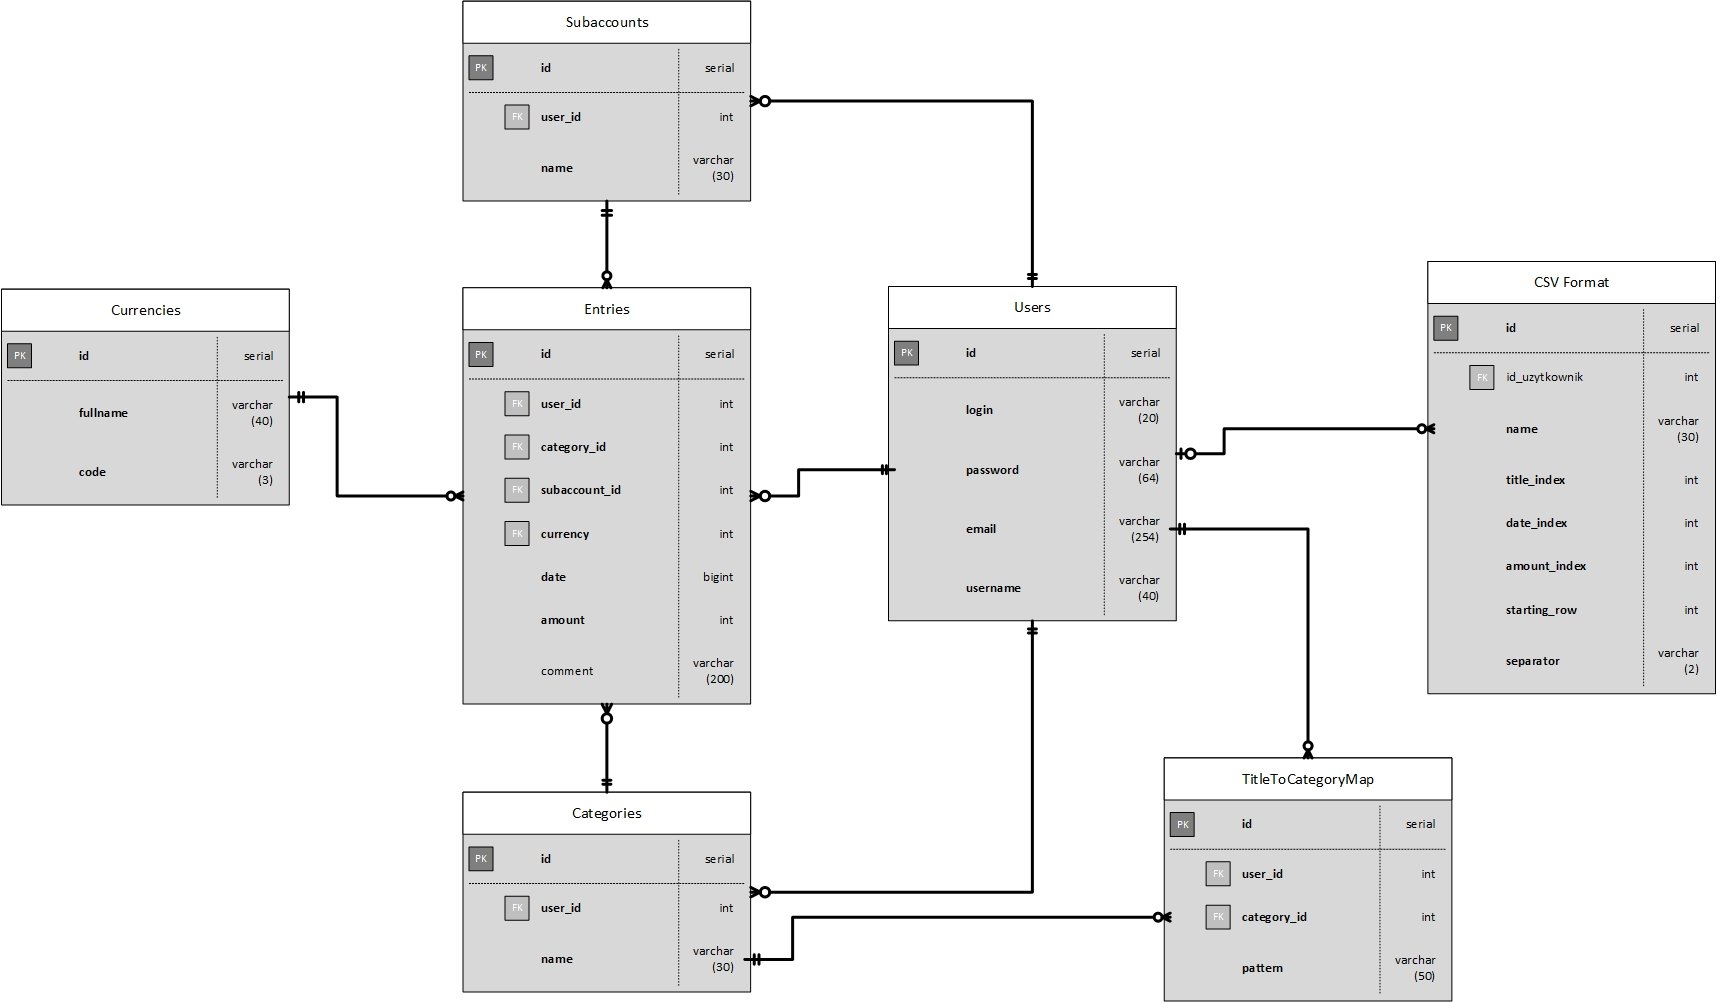
\includegraphics[width=0.8\linewidth]{assets/er.jpg}
		\caption[]{Model związków encji}
		\label{fig:er}
	\end{figure}
	
	Zgodnie z rysunkiem \ref{fig:er}, w bazie danych znajduje się pięć tabel. Tabela \texttt{Użytkownicy} zawiera dane użytkownika takie jak jego login oraz skrót hasła. Tabele \texttt{Subkonta}, \texttt{Układy CSV} oraz \texttt{Kategorie} mają odniesienia do tabeli \texttt{Użytkownicy}, które są opcjonalne w przypadku dwóch wymienionych jako ostatnie. W przypadku braku odniesienia, wpisy te są uznawane jako wspólne (predefiniowane) dla wszystkich użytkowników. Jeden rekord w tabeli \texttt{Wpisy} musi mieć odwołanie do każdej z tabel \texttt{Subkonta}, \texttt{Użytkownicy} oraz \texttt{Kategorie}.
	
	
\end{document}
